\documentclass[12pt]{article}

% Pretty much all of the ams maths packages
\usepackage{amsmath,amsthm,amssymb,amsfonts}

% Allows you to manipulate the page a bit
\usepackage[a4paper]{geometry}

% Pulls the page out a bit - makes it look better (in my opinion)
\usepackage{a4wide}

% Removes paragraph indentation (not needed most of the time now)
\usepackage{parskip}

% Allows inclusion of graphics easily and configurably
\usepackage{graphicx}

% Provides ways to make nice looking tables
\usepackage{booktabs}

% Allows you to rotate tables and figures
\usepackage{rotating}

% Allows shading of table cells
\usepackage{colortbl}
% Define a simple command to use at the start of a table row to make it have a shaded background
\newcommand{\gray}{\rowcolor[gray]{.9}}

\usepackage{textcomp}

% Provides commands to make subfigures (figures with (a), (b) and (c))
\usepackage{subfigure}

% Typesets URLs sensibly - with tt font, clickable in PDFs, and not breaking across lines
\usepackage{url}

% Makes references hyperlinks in PDF output
\usepackage{hyperref}

% Provides ways to include syntax-highlighted source code
\usepackage{listings}
\lstset{frame=single, basicstyle=\ttfamily}

% Provides Harvard-style referencing
\usepackage{natbib}
\bibpunct{(}{)}{;}{a}{,}{,}

% Provides good access to colours
\usepackage{color}
\usepackage{xcolor}

% Simple command I defined to allow me to mark TODO items in red
\newcommand{\todo}[1] {\textbf{\textcolor{red}{#1}}}

% Allows fancy stuff in the page header
\usepackage{fancyhdr}
\pagestyle{fancy}

% Vastly improves the standard formatting of captions
\usepackage[margin=10pt,font=small,labelfont=bf, labelsep=endash]{caption}

% Standard title, author etc.
\title{Report: Sudoku}
\author{by	Karina Abramova,\\ Mikkel Bernt Buchvardt \\ and\\ Theodor Lars Nyholm Ommen}
\date{}
% Put text on the left-hand and right-hand side of the header
\fancyhead{}
\lhead{Sudoku}
\rhead{Abramova - Buchvardt - Ommen}
\chead{}

\usepackage{titletoc}

\renewcommand{\thepart}{\Alph{part}}

\renewcommand{\thesection}{\arabic{section}}
\renewcommand{\thesubsection}{\alph{subsection})}
\renewcommand{\thesubsubsection}{\alph{subsection}\alph{subsubsection})}

\titlecontents{chapter}
[2.65em]
{\addvspace{10pt}\bfseries}
{\contentslabel{2.3em}}
{\hspace*{-2.3em}}
{\space.\hfill\contentspage}


\definecolor{dkgreen}{rgb}{0,0.6,0}
\definecolor{gray}{rgb}{0.5,0.5,0.5}
\definecolor{mauve}{rgb}{0.58,0,0.82}

\lstset{frame=tb,
	language=Java,
	aboveskip=3mm,
	belowskip=3mm,
	showstringspaces=false,
	columns=flexible,
	basicstyle={\small\ttfamily},
%	numbers=left,
	numberstyle=\tiny\color{gray},
	keywordstyle=\color{blue},
	commentstyle=\color{dkgreen},
	stringstyle=\color{mauve},
	breaklines=true,
	breakatwhitespace=true,
	tabsize=3
}

\begin{document}


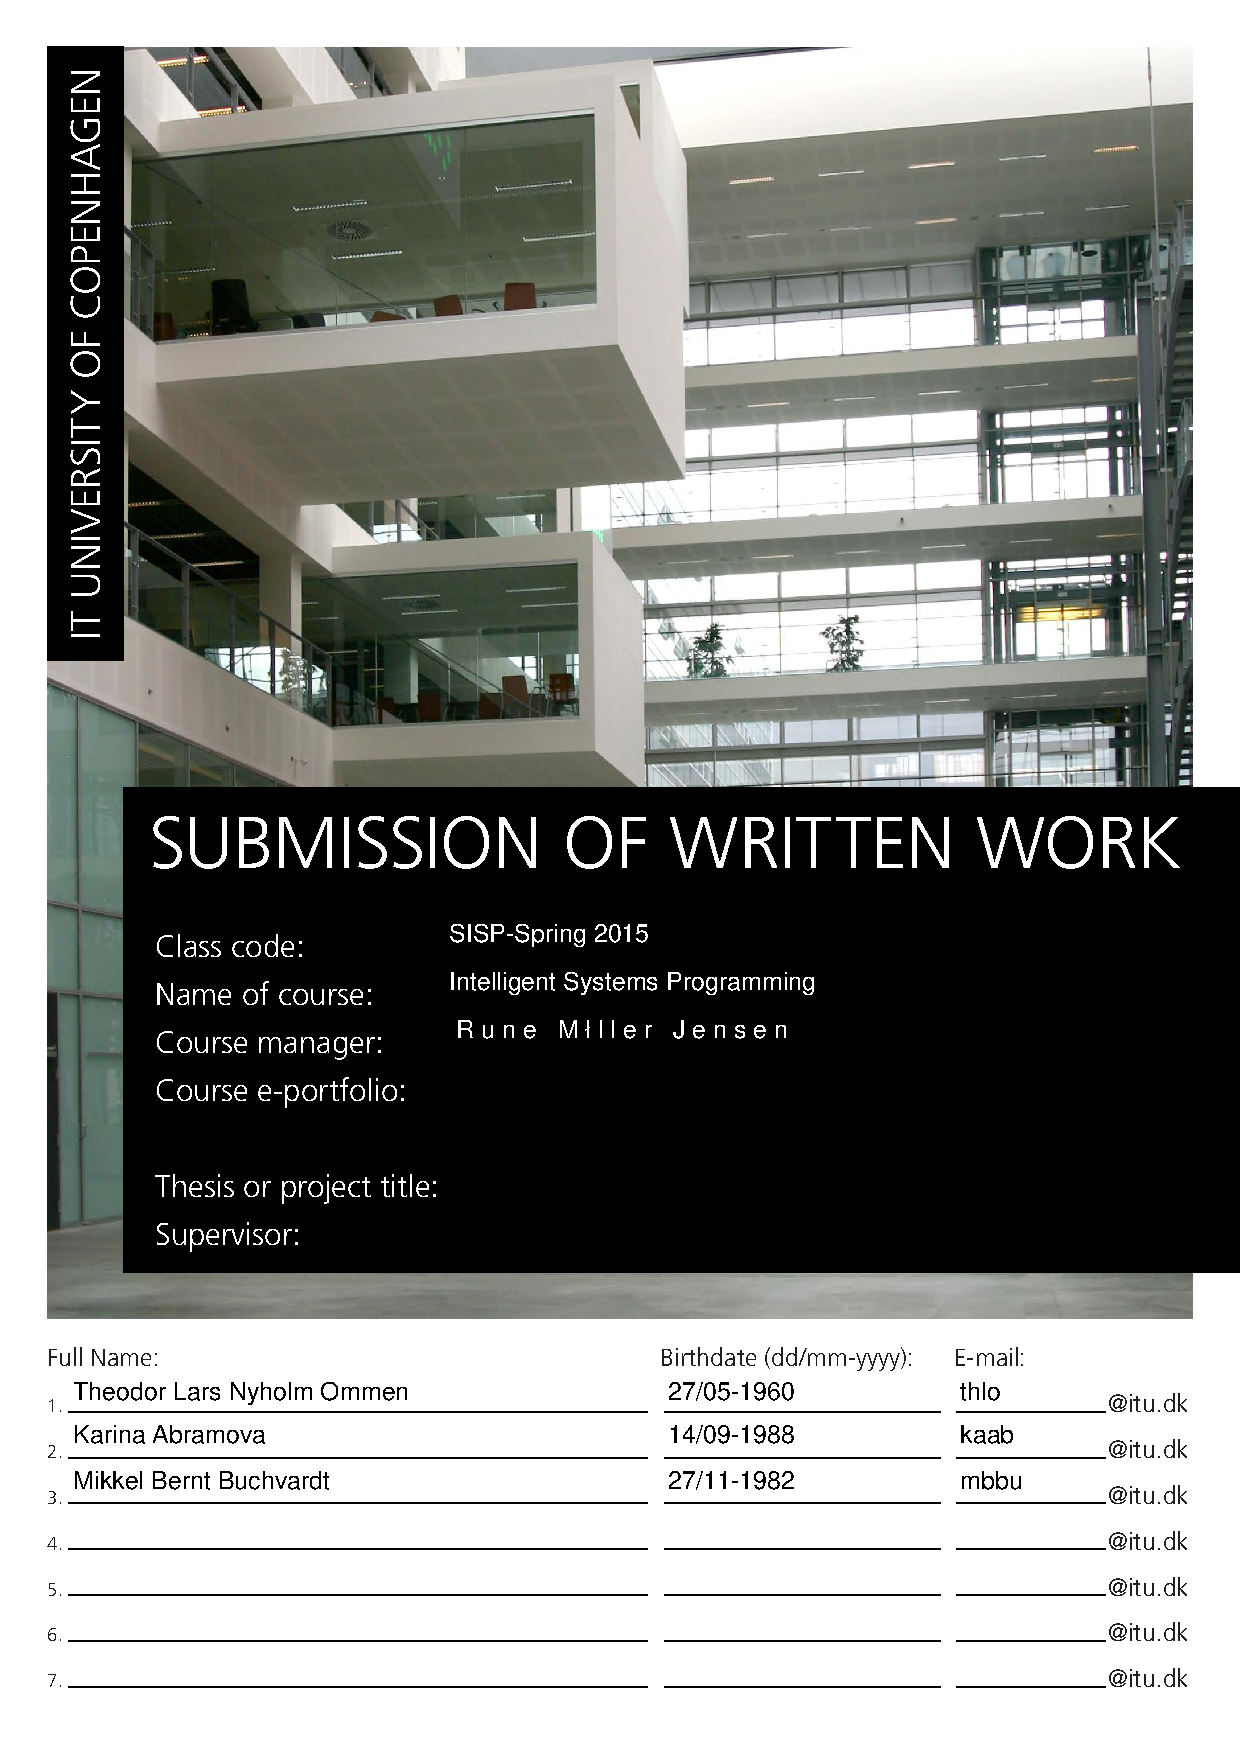
\includegraphics[scale=0.7]{./frontpage}

\begingroup
\let\flushleft
\let\endcenter\endflushleft
\maketitle
\endgroup



\section{Introduction}

[4, 0, 0, 2, 0, 8, 0, 0, 3, 0, 0, 1, 0, 0, 0, 9, 0, 0, 0, 7, 0, 0, 9, 0, 0, 2, 0, 6, 0, 0, 3, 0, 0, 0, 0, 8, 0, 0, 5, 0, 0, 0, 1, 0, 0, 8, 0, 0, 0, 0, 9, 0, 0, 5, 0, 5, 0, 0, 3, 0, 0, 9, 0, 0, 0, 7, 0, 0, 0, 3, 0, 0, 2, 0, 0, 9, 0, 4, 0, 0, 6]



\section{Rules}

As described in the assignment there are two rules to be observed:
\begin{itemize}
	\item On an N by N size board N queens has to be placed
	\item All queens are to be considered able to of different color
\end{itemize}

We had to find a way to translate these two rules into boolean functions.

There has to be exactly one queen in each row and each column
In each diagonal there can also be only one queen.

Another way of describing the exactly one queen in each row is by saying that if there is a queen in the first cell, there cannot be one in the second and there cannot be one in the third and so on.
These rules have to be entered in the BDD and only then can you start placing queens on the board (and in the BDD).

\section{Code}


For setting expression on where a queen can be placed we set up the BDD with nand expressions for all fields depending on each other (if the first then not the second and not the third and so on).



For instance the code for the expression that only one cell in a column can contain a queen is done as follows(from line 121 in QueensLogic.java):

\begin{lstlisting}
         /* No one in the same column */
         for (l = 0; l < N; l++) {
         if (l != j) { // if it is not the same variable
         BDD u = X[i][l].apply(X[i][j], BDDFactory.nand); 
         // creating tmp BDD by applying the binary operator opr NOT AND to the two BDDs.
         // ie. (0 and not 5 and not 10 and not 15 and not 20  ) for the first column
         //     (1 and not 6 and not 11 and not 16 and not 21) for the seconnd row ... (for N=5)
         a.andWith(u);
         }
\end{lstlisting}

The other rules are entered into the BDD in the same way and they are finally and'ed to each other in one BDD called queen.

'queen' is now a BDD representing all the rules an is ready for restrictions (the placing of queens in different cells).

In order to ensure that no queen placed on the board will violate any of the rules we looked at BDD.pathCount() method for the BDD 'queen' restricted to the placement of a queen (what actually happens to the BDD when a queen is placed at a specific field on the board?). 

In details it is done by the insertQueen() method that inserts a queen by restricting the variable that corresponds to the cell to the BDD queen and then iterate through every cell on the board. By temporary restricting every cell to the resulting BDD of the placement and checking if there exists a path with this restriction it can be determined if the cell should be crossed or stay open.


\section{User Interface}

We used a print of the board to the console for debugging and used the GUI for the final version. We kept the console printouts to make it easier to understand what is actually going on. 
 
We decided not to build in means of termination in to the program as the user will want to see the result of the configuration.


\end{document}